\lab{Algorithm}{Compressed Sensing}{Compressed Sensing}
\label{Ch:CS}

\objective{Learn About Techniques in Compressed Sensing.}


One of the more important and fundamental problems in mathematics and science is solving a system of linear equations
\[
Ax = b.
\]
Depending on the properties of the matrix $A$ (such as its dimensions and rank), there may be exactly one
solution, infinitely many solutions, or no solution at all. 

In the case where $A$ is a square invertible matrix, there is of course one unique solution, given by
$A^{-1}b$. There are various computational methods for inverting $A$, and we have studied many of them previously.

When $b$ does not lie in the range of $A$, there is no exact solution. We can still hope to find approximate solutions,
and techniques such as least squares and least absolute deviations provide ways to do this.

The final case is when there are infinitely many vectors $x$ that satisfy $Ax = b$. How do we decide which vector
to choose? A common approach is to choose a vector $x$ of minimal norm satisfying $Ax = b$. This can be stated as 
an optimization problem:
\begin{align*}
\text{minimize}\qquad &\|x\|\\
\text{subject to} \qquad &Ax = b.
\end{align*}

When we use the standard Euclidean $2$-norm, the problem is equivalent to the quadratic program
\begin{align*}
\text{minimize}\qquad &x^Tx\\
\text{subject to} \qquad &Ax = b,
\end{align*}
which we can solve using an iterative procedure. Alternatively, the solution is given directly by $A^\dagger b$,
where $A^\dagger$ is the Moore-Penrose pseudoinverse of $A$. 

If instead of the $2$-norm we use the $1$-norm, our problem can be restated as a linear program, and solved
efficiently using the Simplex Algorithm or an Interior Point method. Of course we can use any norm whatsoever, but
finding the solution may be much more difficult.

The basic problem in the field of Compressed Sensing is to recover or reconstruct certain types of signals
from a small set of measurements. For example, we might have measurements of the frequency spectrum of an
audio signal, and we wish to recover the original audio signal as nearly as possible. Mathematically, this
problem can be viewed as solving the under-determined system of equations
$Ax = b$, where $b$ is a vector of measurements and $A$ is called the measurement matrix.
The crucial idea that Compressed Sensing brings to the table is the concept of \emph{sparsity}, which we address now.

\section*{Sparsity and the $l_0$ Pseudonorm}
\emph{Sparsity} is a property of vectors in $\mathbb{R}^n$ related to how compactly and concisely they can
be represented in a given basis. Stated more concretely, the sparsity of a vector $x$ (expressed in some given
basis) refers to how many nonzero entries are in $x$. A vector having at most $k$ nonzero entries is said to be
$k$-sparse. This concept can be extended to time series (such as an audio signal) and to images. Figure 32.1 shows
examples of both sparse and non-sparse signals.

\begin{figure}
\centering
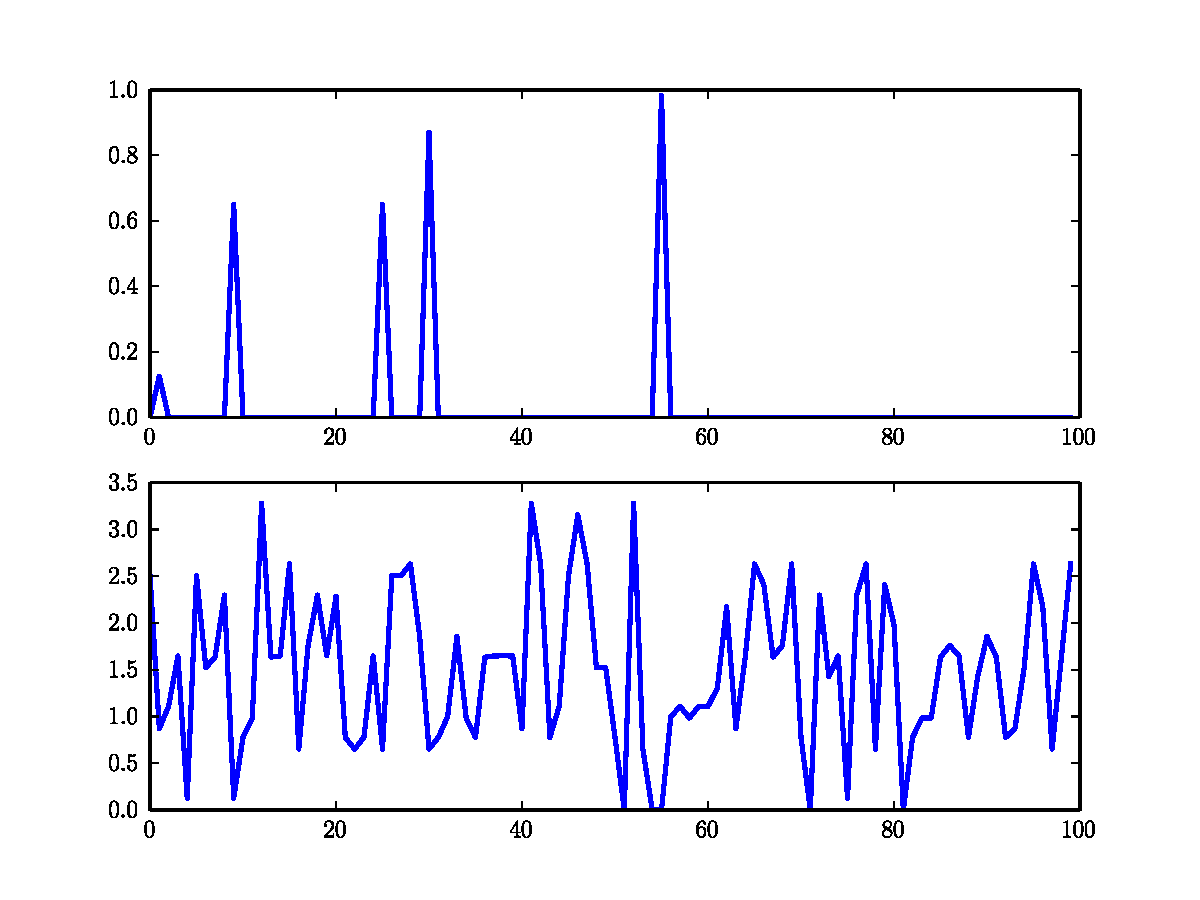
\includegraphics[width=\textwidth]{sparse.pdf}
\caption{A sparse signal and a non-sparse signal.}
\label{fig:sparse}
\end{figure}

As a convenient way of measuring sparsity, we define the so-called $l_0$ pseudonorm, notated $\|\cdot\|_0$,
that simply counts the number of nonzero entries in a vector. For example, if we have
\[
x = 
\begin{bmatrix}
1&0&0&-4&0
\end{bmatrix}^T
\]
and
\[
y = 
\begin{bmatrix}
.5&.2&-.01&3&0
\end{bmatrix}^T,
\]
we then have
\[
\|x\|_0 = 2
\]
and
\[
\|y\|_0 = 4.
\]
Despite our choice of notation, $\|\cdot\|_0$ is not truly a norm (which properties does it fail to satisfy?).
Keep this in mind, even if we refer to it as the $l_0$ norm. 

As mentioned earlier, sparsity is of central importance in Compressed Sensing, for it provides a way for us to 
select from the infinite possibilities a single vector $x$ satisfying $Ax = b$. In particular, we require $x$ to 
be as sparse as possible, i.e. to have minimal $l_0$ norm. Stated explicitly as an optimization problem, Compressed
Sensing boils down 
\begin{align*}
\text{minimize}\qquad &\|x\|_0\\
\text{subject to} \qquad &Ax = b.
\end{align*}

\section*{Sparse Reconstruction}
How does the Compressed Sensing framework laid out above help us recover a signal from a set of measurements? 
If we know nothing about the signal that we are trying to reconstruct, anything but a complete set of measurements
(or \emph{samples}) of the signal will be insufficient to fully recover the signal without any error. 

However, we can often make certain assumptions about the unknown signal, such as setting an upper bound for
its highest frequency. Given this prior knowledge about the frequency of the signal, we \emph{are} able to 
perfectly or nearly perfectly reconstruct the signal from an incomplete set of measurements, provided that
the sampling rate of the measurements is more than twice that of the largest frequency. This classic result
in signal processing theory is known as the \emph{Nyquist-Shannon sampling theorem}.

What if, instead of having prior knowledge about the frequency of the signal, we have prior knowledge about
its sparsity? Recent research asserts that it is possible to recover sparse signals to great accuracy from just 
a few measurements. This matches intuition: sparse signals do not contain much information, and so it ought to
be possible to recover that information from just a few samples. Stated more precisely, if $\hat{x} \in \mathbb{R}^n$ 
is sufficiently sparse and an $m \times n$ matrix $A$ ($m < n$) satisfies certain properties (to be described later),
with $A\hat{x} = b$, then the solution of the optimization problem
\begin{align*}
\text{minimize}\qquad &\|x\|_0\\
\text{subject to}\qquad &Ax = b
\end{align*}
yields $\hat{x}$. 

The matrix $A$ above must satisfy a technical condition called the \emph{Restricted Isometry Principle}. Most
random matrices obtained from standard distributions (such as the Gaussian or Bernoulli distributions) satisfy this
condition, as do transformation matrices into the Fourier and Wavelet domains. Generally speaking,
the measurement matrix $A$ represents a change of basis from the \emph{sparse} basis to the \emph{measurement} basis, 
followed by an under-sampling of the signal. The Restricted Isometry Principle guarantees that the measurement
basis is incoherent with the sparse basis; that is, a sparse signal in the sparse basis is diffuse in the measurement
basis, and vice versa (see Figure \ref{fig:incoherent}). This ensures that the information contained in the few nonzero
coefficients in the sparse
domain is spread out randomly and roughly evenly among the coefficients in the measurement domain. 
We can then obtain a small random subset of these measurement coefficients, solve the above optimization problem,
and recover the original signal. 

\begin{figure}
\centering
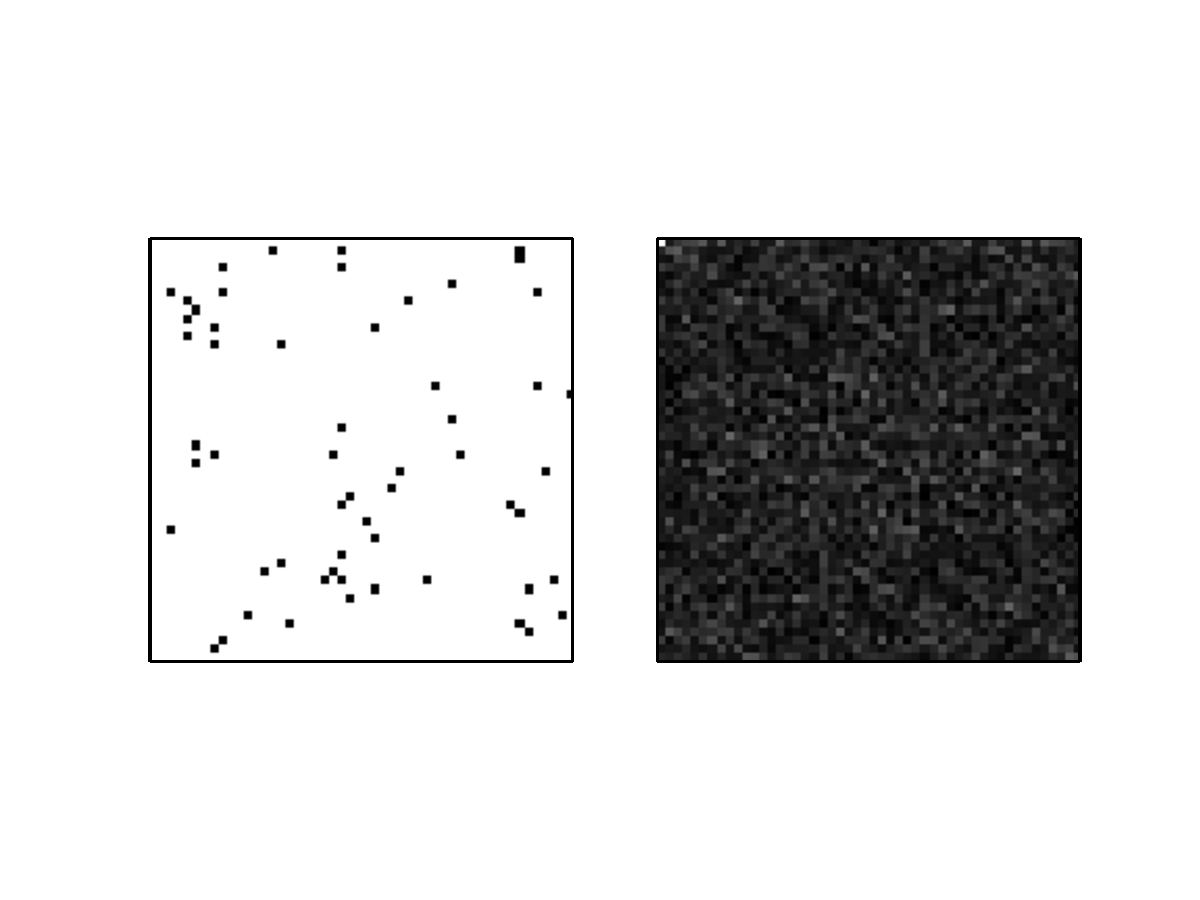
\includegraphics[width=\textwidth]{incoherent.pdf}
\caption{A sparse image (left) and its Fourier transform (right). The Fourier domain is incoherent with the 
standard domain, so the Fourier transform of the spare image is quite diffuse.}
\label{fig:incoherent}
\end{figure}

Fortunately, many types of signals that we wish to measure are sparse in some domain. For example, many images
are sparse in the Wavelet domain. It turns out that the Fourier domain is incoherent with the Wavelet domain,
so if we take measurements of the image in the Fourier domain, we are able to recover the image with high 
fidelity from relatively few measurements. This has been particularly useful in magnetic resonance imaging 
(MRI), a medical process that obtains pictures of tissues and organs in the body by taking measurements in
the Fourier domain. Collecting these measurements can in some cases be harmful. Compressed sensing
allows for fewer measurements and therefore a shorter, safer MRI experience.

\section*{Solving the $l_0$ Minimization Problem}
Now that we have become familiar with the mathematical underpinnings of compressed sensing, let us now turn to 
actually solving the problem. Unfortunately, the $l_0$ minimization problem stated above is NP hard and thus 
computationally intractable in its current form. Another key result in compressed sensing states that we can
replace the $l_0$ norm with the $l_1$ norm and with high probability still recover the original signal, provided
it is sufficiently sparse. Since the $l_1$ minimization problem can be solved efficiently, we have a viable 
computational approach to compressed sensing. 

Recall that we can convert the $l_1$ minimization problem into a linear program by introducing an additional
vector $u$ of length $n$, and then solving
\begin{align*}
\text{minimize}\qquad 
&\begin{bmatrix}
\mathbf{1} & 0
\end{bmatrix}
\begin{bmatrix}
u \\
x
\end{bmatrix}\\
\text{subject to}\qquad
&\begin{bmatrix}
-I & I\\
-I & -I
\end{bmatrix}
\begin{bmatrix}
u \\
x
\end{bmatrix}
\leq 
\begin{bmatrix}
0\\
0
\end{bmatrix},\\
&\begin{bmatrix}
0 & A
\end{bmatrix}
\begin{bmatrix}
u \\
x
\end{bmatrix}
= 
b.
\end{align*}
Of course, solving this gives values for the optimal $u$ and the optimal $x$, but we only care about the optimal $x$.

\begin{problem}
Write a function \li{l1Min} that takes a matrix $A$ and vector $b$ as inputs, and returns the solution to the 
optimization problem 
\begin{align*}
\text{minimize}\qquad &\|x\|_1\\
\text{subject to} \qquad &Ax = b.
\end{align*}
Formulate the problem as a linear program, and use CVXOPT to obtain the solution.
\end{problem}

Let's reconstruct a sparse image using different numbers of measurements, and compare results.
Load the image contained in the file \li{ACME.png} into Python as follows:
\begin{lstlisting}
>>> import numpy as np
>>> from matplotlib import pyplot as plt
>>> acme = 1 - plt.imread('ACME.png')[:,:,0]
>>> acme.shape
(32L, 32L)
\end{lstlisting}
The image contains $32^2$ pixels, and so viewed as a flat vector, it has $32^2$ entries.
Now build a random measurement matrix based on $m$ samples as follows:
\begin{lstlisting}
>>> # assume the variable m has been initialized
>>> np.random.seed(1337)
>>> A = np.random.randint(0,high=2,size=(m,32**2))
\end{lstlisting}
Next, calculate the $m$ measurements:
\begin{lstlisting}
>>> b = A.dot(acme.flatten())
\end{lstlisting}
We are now ready to reconstruct the image using our function \li{l1Min}:
\begin{lstlisting}
>>> rec_acme = l1Min(A,b)
\end{lstlisting}

\begin{problem}
Following the example above, reconstruct the ACME image using 200, 250, and 270 measurements.
Be sure to execute the code \li{np.random.seed(1337)} prior to each time you initialize
your measurement matrix, so that you will obtain consistent answers. Report the $2$-norm
distance between the each reconstructed image and the original ACME image. 
\end{problem}

Figure \ref{fig:reconstruct} shows the results of reconstructing a similar sparse image using both the $1$-norm and 
the $2$-norm.

\begin{figure}
\centering
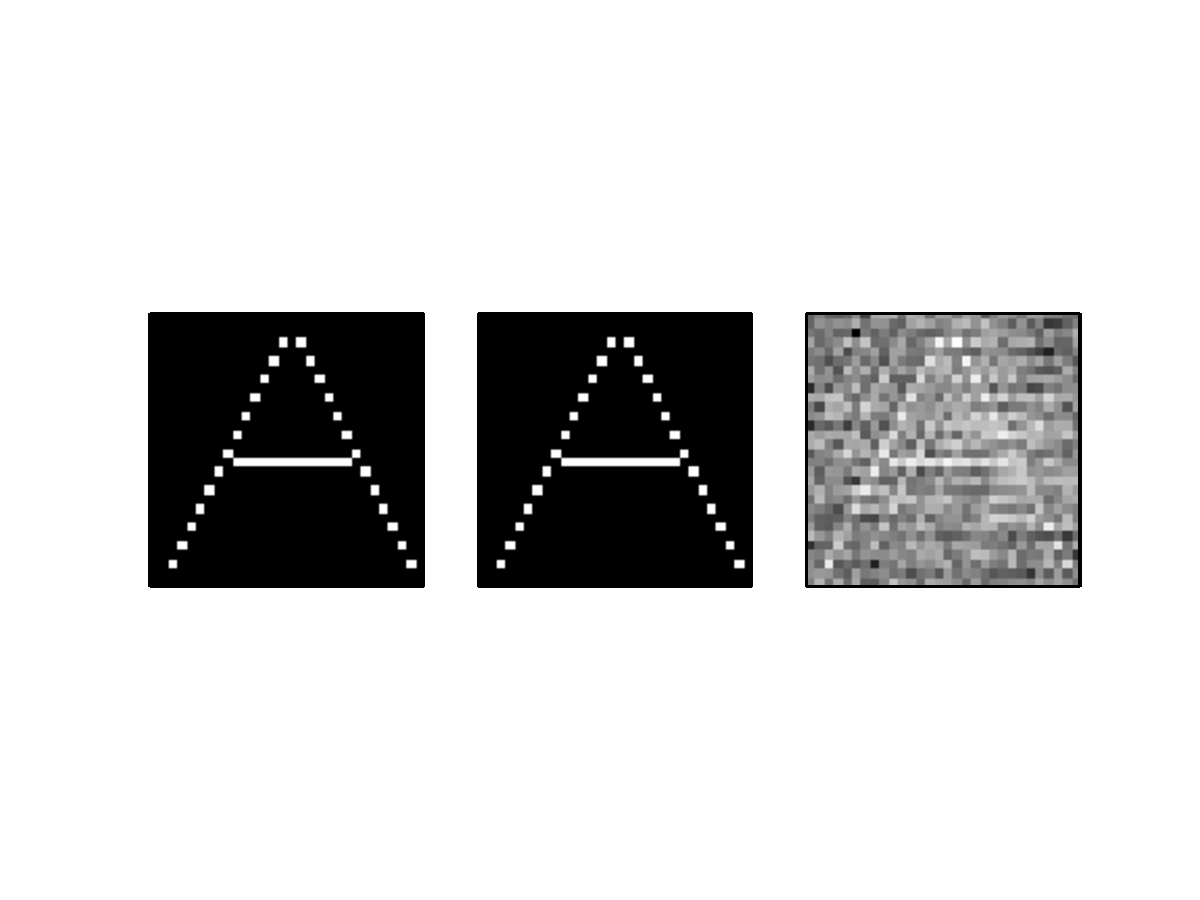
\includegraphics[width=\textwidth]{reconstruct.pdf}
\caption{A sparse image (left), perfect reconstruction using $l_1$ minimization (middle),  and
imperfect reconstruction using $l_2$ minimization (right).}
\label{fig:reconstruct}
\end{figure}
\section*{Tesselated Surfaces and the Single Pixel Camera}
We now generalize our discussion to reconstructing functions defined on surfaces. Such a function might
give a color at each point on the surface, or the temperature, or some other property. The surface may be 
a sphere (to model the surface of the earth), a cube, or some other desired form. To make the problem 
tractable, we must break the surface up into a set of discrete polygonal faces, called a tessellation. See
Figure \ref{Fig:Earth} for an example of a tessellated sphere.

Now that we have a tessellation, our function can be represented by a vector, consisting of the function value 
for each facet (element of the tessellation). We are thus in a position to apply the techniques of compressed
sensing to recover the function. 

How do we go about acquiring color measurements on a tessellated surface? One cheap method is to use a \emph{single-pixel
camera}. Such a camera can only measure color value at a time. The camera points to a specific spot on the surface, and
records a weighted average of the colors near that spot. By taking measurements at random spots across the surface,
the single-pixel camera provides us with a vector of measurements, which we can then use to reconstruct the color value for
each facet of the tessellation. See Figure \ref{Fig:Earth} for the results of a single-pixel camera taking measurements of the earth.

\begin{figure}
\begin{center}
$\begin{array}{cc}
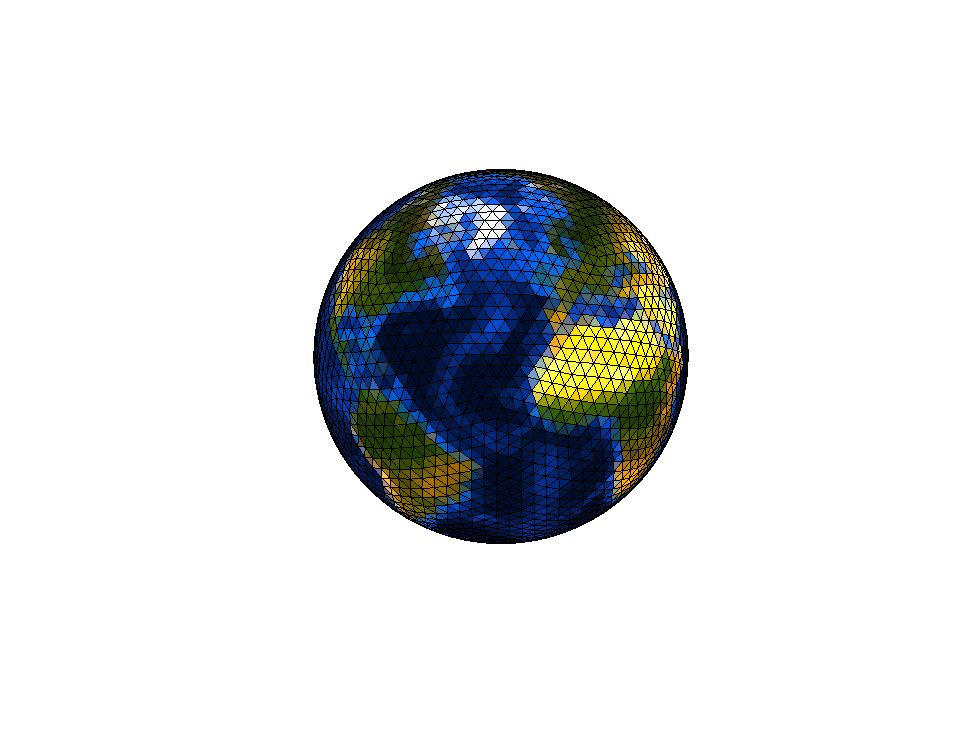
\includegraphics[scale = .6]{OriginalCropped} &
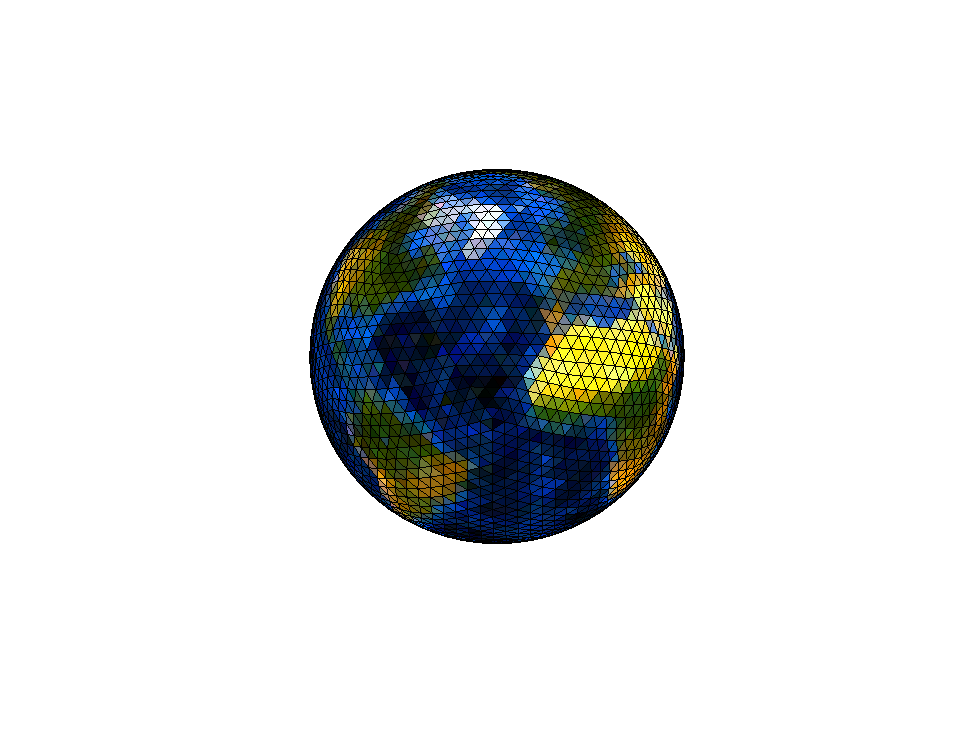
\includegraphics[scale = .6]{EstimatedCropped} \\
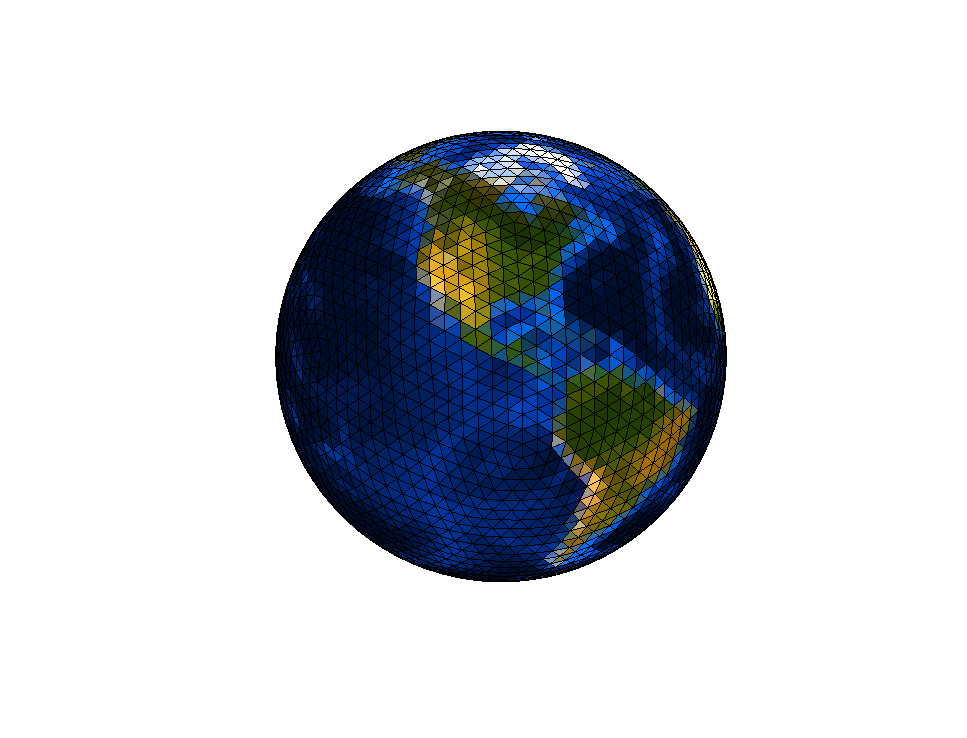
\includegraphics[scale = .5]{Original2Cropped} &
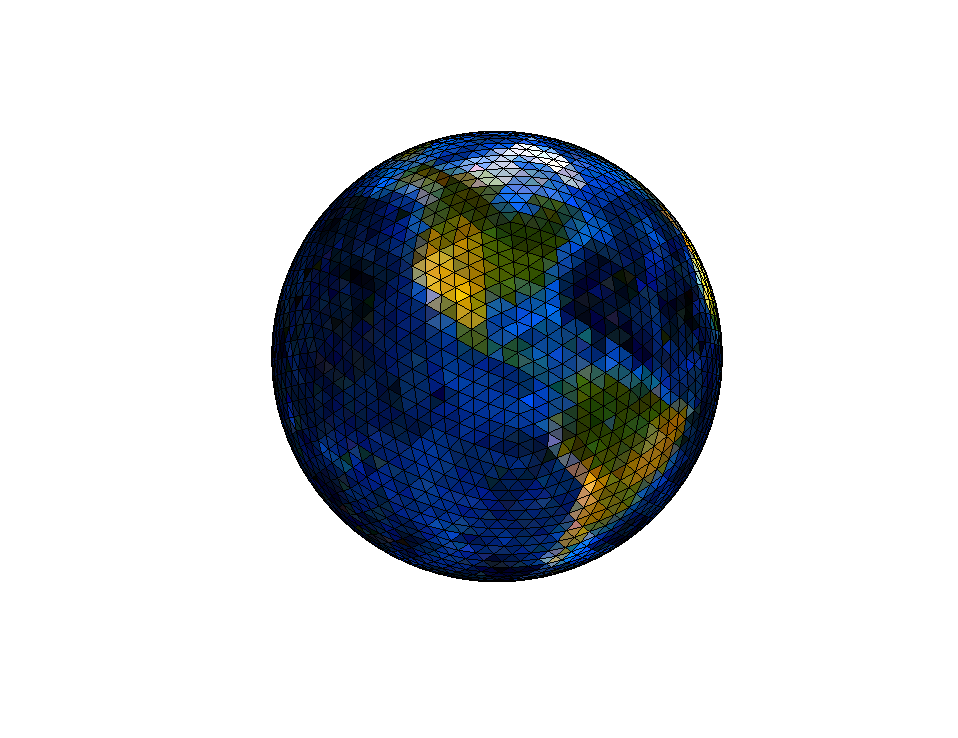
\includegraphics[scale = .5]{Estimated2Cropped} \\
\mbox{\bf (a)} & \mbox{\bf (b)}
\end{array}$
\end{center}
\caption{A 3-D model of the earth, with 5120 faces. $(a)$ shows two views of the model drawn directly from satellite imagery. $(b)$ shows two views of the reconstruction based upon 2500 single-pixel measurements.}
\label{Fig:Earth}
\end{figure}

The single-pixel camera measurement process can be modeled as matrix multiplication
by a measurement matrix $A$, which fortunately has the Restricted Isometry Property. In the following,
we provide you with code to take single pixel measurements. It works as follows 
\begin{lstlisting}
run camera.py
myCamera=Camera(faces,vertices,colors)
\end{lstlisting}
Where faces, verticies and colors are given by the tesselation. To take a picture you use 
\begin{lstlisting}
myCamera.add_pic(theta,phi,r)
\end{lstlisting}
Where theta, phi, and r are the spherical coordinates of the camera. Recall to change spherical coordinates to rectangular the formula is   
\[
(r\sin(\phi)\cos(\theta),r\sin(\phi)\sin(\theta),r\cos(\phi))
\]
Where $\theta \in [0,2\pi),\phi \in [0,\pi), r \in [0,\infty)$

Calling \li{add_pic} many times at different places on a sphere (constant $r$ value, varying $\theta$ and $\phi$) will build the measurement matrix as well as the measurements. You can return these by
\begin{lstlisting}
A,b=myCamera.returnData()
\end{lstlisting}

In this applications signals are only sparse in some appropriate representation (such as Fourier or wavelet). This method generally can still be applied in such cases. Let $V$ represent the transformation under which $s$ is sparse, or in other words:
\begin{equation}
s = V p
\end{equation}
$V$ is the inverse Fourier. We can then recast $A s=b$ as
\begin{equation}
A V p = b
\end{equation}
This then allows us to find $p$ using Compressed Sensing, which in turn allows us to reconstruct $s$ by using $V$. In the the following problem $V$ will be given to you.

You must reconstruct the color functions
for the tesselated surfaces, and then plot these surfaces using the code we provide you.

%\begin{problem}
%We will perform compressed sensing on a Rubik's cube. The Rubik's cube has a natural tessellation, with each facet
%being a square having one color. Each color can be represented as a vector of length 3, where we have split the
%color into three color channels (red, green, and blue). The set of colors for the entire Rubik's cube is fairly
%sparse in each color channel, so we can reconstruct the color values in each color channel separately.
%
%In the file \li{StudentRubiksData.npz}, we have given you the measurement matrices for each color channel
%(accessed by the keys \li{'A1', 'A2', 'A3'}) along with the respective measurements in each color channel
%(accessed by the keys \li{'b1', 'b2', 'b3'}). Reconstruct the colors in each color channel, obtaining
%three arrays. Then stack these arrays row-wise into an array with three rows. Report this final array.
%
%To visualize your result, we have provided code in the file \li{visualize.py} that you can call.
%You also need to load in the array corresponding to the key \li{'centers'} in the data archive
%\li{StudentRubiksData.npz}. We assume the variable holding this array is named \li{c}.
%Execute the following (assuming that the variable holding the array
%you obtained above containing the reconstructed colors is named \li{r}):
%\begin{lstlisting}
%>>> from visualize import visualizeSurface
%>>> visualizeSurface(r.clip(0,1), c, 3)
%\end{lstlisting}
%You should see a plot showing the Rubik's cube.
%\end{problem}

\begin{problem}
We will reconstruct the surface of the earth from sparse satellite imagery. The earth is modeled by a sphere,
which can be tessellated into triangular faces, each having a color value. There are three color 
channels, and the colors are sparse in each channel in the appropriate basis. 

In the file \li{StudentEarthData.npz}, we have given you the faces, vertices, colors, and the inverse fourier matrix, (accessed by the key \li{'faces'}, \li{'vertices'}, \li{'C'}, and \li{'V'} respectively), Take pictures with the single pixel camera code (using $r=3$) and then reconstruct the colors in each color channel, obtaining
three arrays. Then stack these arrays column-wise into an array with three columns. Report this final array.

To visualize your result, we have provided code in the file \li{visualize2.py} that you can call.
Execute the following (assuming that the variable holding the array
you obtained above containing the reconstructed colors is named \li{s}):
\begin{lstlisting}
>>> from visualize2 import visualizeEarth
>>> visualizeEarth(faces, vertices, s.clip(0,1))
\end{lstlisting}
You should see a plot showing the reconstructed earth. We could have reconstructed a more detailed earth by choosing a finer tessellation, but you should be able to make out the shapes of the major continents. You can compare this to the original by running
\begin{lstlisting}
>>> visualizeEarth(faces, vertices, colors)
\end{lstlisting}

Try the reconstruction with 450, 550, 650 measurements and report the absolute difference between the reconstruction and the actual colors.
\end{problem}